\chapter*{Interpolazione}\label{cap:interpolazione}

Come accennato nel capitolo \ref{cap:parametri}, la frequenza di campionamento e il numero di campioni estratti per frame non garantiscono la precisione desiderata.
La soluzione introdotta per aumentare tale precisione è interpolare i valori attorno al massimo trovato.
L'interpolazione utilizzata è di tipo \emph{spline}.
Sono stati interpolati ventuno punti, di cui nove con ascissa inferiore a quella del massimo, il massimo stesso e undici con ascissa superiore al massimo.

	\begin{figure}[h]
	  \begin{center} 
	    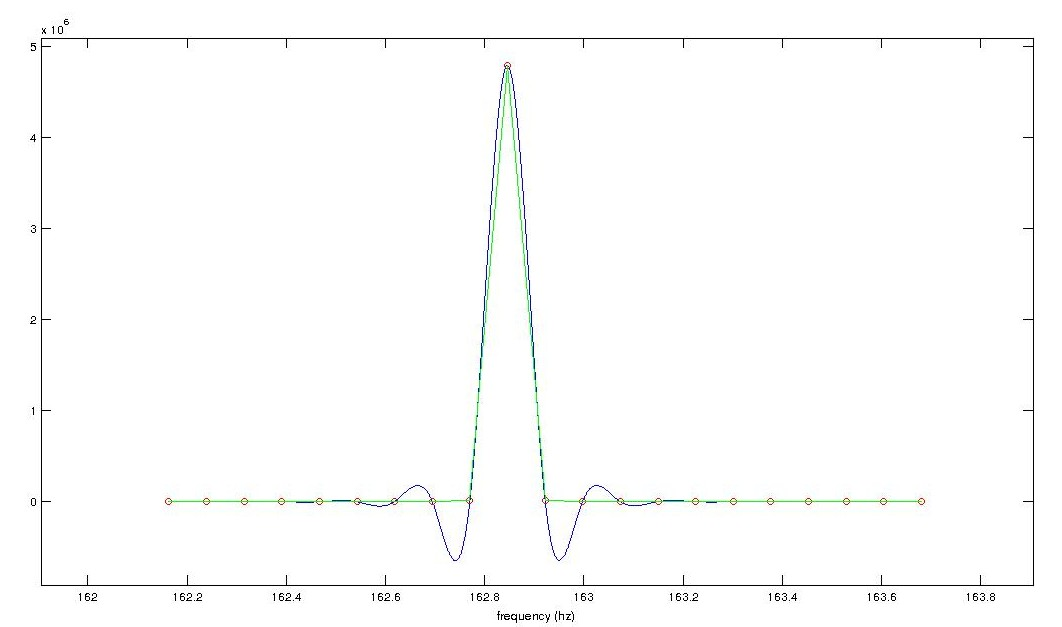
\includegraphics[width=\textwidth*\real{0.9}]{images/ch_05/interpolazione.jpg}
	  \end{center} 
	  \caption{\textit{Interpolazione per migliorare la ricerca del massimo}}  
	  \label{fig:interpolazione}
	\end{figure}

La figura \ref{fig:interpolazione} mostra un esempio di interpolazione. 
I punti evidenziati in rosso, rappresentano il prodotto delle versioni sotto-campionate dello spettro del segnale audio.
La linea verde che li congiunge, rappresenta un'interpolazione lineare.
La linea blu che passa per tutti i punti rappresenta l'interpolazione spline realizzata al fine di trovare il massimo della funzione con una maggiore precisione.

Successivamente all'interpolazione, l'operazione di ricerca del massimo viene effettuata nuovamente e l'ascissa del punto trovato viene utilizzata come frequenza della nota suonata dalla corda della chitarra.
